\documentclass[a4paper,12pt]{article}

\usepackage{graphicx} % Required for inserting images
\usepackage{amsmath,amssymb,amsfonts}
\usepackage{subcaption}
% Use Times New Roman font
\usepackage{times}
\usepackage[a4paper, top=1in, bottom=0.8in, left=1.1in, right=0.8in]{geometry}
\usepackage{float}
\usepackage{listings}
\usepackage{xcolor} % For customizing code colors
\setlength{\parindent}{0pt}
\usepackage{titlesec} % Add this to your preamble
\titleformat{\section}
{\normalfont\large\bfseries}{\thesection}{1em}{}
% Set spacing for sections
\titlespacing*{\section}
{0pt}  % Left spacing
{1ex} % Space before (adjust this value)
{1ex}  % Space after (adjust this value)
\begin{document}
	\section{Experiment No. 10}
	
	
	\section{Experiment Title }
	Design and Analyze a 4 Bit ALU on MICROWIND 3.0
	\section{Objective}
	The main objectives of this report are:
	\begin{itemize}
	\item 	To design and implement a 4-bit Arithmetic Logic Unit (ALU) using nMOS pass transistor logic
	
	\end{itemize}
	\section{Theory}
	
	A 4-bit Arithmetic Logic Unit (ALU) is a critical component of digital systems, designed to perform fundamental arithmetic and logical operations. In this experiment, the ALU is built using nMOS pass transistor logic to implement various functions, including addition, subtraction, and basic logical operations such as AND, OR, and XOR. The use of nMOS pass transistor logic provides a compact and efficient design approach, making it suitable for integration in digital circuits. The functionality and performance of the ALU are explored in detail during this study.\\
	For any column $k$ of a binary adder, there are three inputs: the corresponding bits of the input numbers $A_k$ and $B_k$, and the `previous carry' $C_{k-1}$. There are two outputs: the sum $S_k$ and the new carry $C_k$. The truth table for the $k$-th column of the binary adder is shown in Table~\ref{table:truth-table}.
	
	\begin{table}[h!]
		\centering
		\caption{Truth table for binary adder}
		\label{table:truth-table}
		\begin{tabular}{|c|c|c||c|c|}
			\hline
			\multicolumn{3}{|c||}{\textbf{Inputs}} & \multicolumn{2}{c|}{\textbf{Outputs}} \\
			\hline
			$A_k$ & $B_k$ & $C_{k-1}$ & $S_k$ & $C_k$ \\
			\hline
			0 & 0 & 0 & 0 & 0 \\
			0 & 1 & 0 & 1 & 0 \\
			1 & 0 & 0 & 1 & 0 \\
			1 & 1 & 0 & 0 & 1 \\
			0 & 0 & 1 & 1 & 0 \\
			0 & 1 & 1 & 0 & 1 \\
			1 & 0 & 1 & 0 & 1 \\
			1 & 1 & 1 & 1 & 1 \\
			\hline
		\end{tabular}
	\end{table}
		For any column $k$ of a binary adder, there are three inputs: the corresponding bits of the input numbers $A_k$ and $B_k$, and the `previous carry' $C_{k-1}$. There are two outputs: the sum $S_k$ and the new carry $C_k$. The truth table for the $k$-th column of the binary adder is shown in Table~\ref{table:truth-table}.
	
	\noindent
	Standard adder equations, which fully describe the entries in Table~\ref{table:truth-table}, are as follows:
	
	\begin{align*}
		S_k &= H_k \overline{C}_{k-1} + \overline{H_k} C_{k-1}, \\
		C_k &= A_k B_k + H_k C_{k-1},
	\end{align*}
	where $H_k$ is the \textit{half-sum}, defined as:
	\[
	H_k = \overline{A_k}B_k + A_k\overline{B_k}.
	\]
	
	Here, $C_{k-1}$ represents the previous carry, with $0 \leq k \leq n-1$ for $n$-bit numbers. These equations can be directly implemented using \textsc{AND-OR} functions or, more economically, with \textsc{Exclusive-Or} gates.
	
	For custom implementations, restating the requirements in another way may be advantageous. 
	\begin{figure}[H]
		\centering
		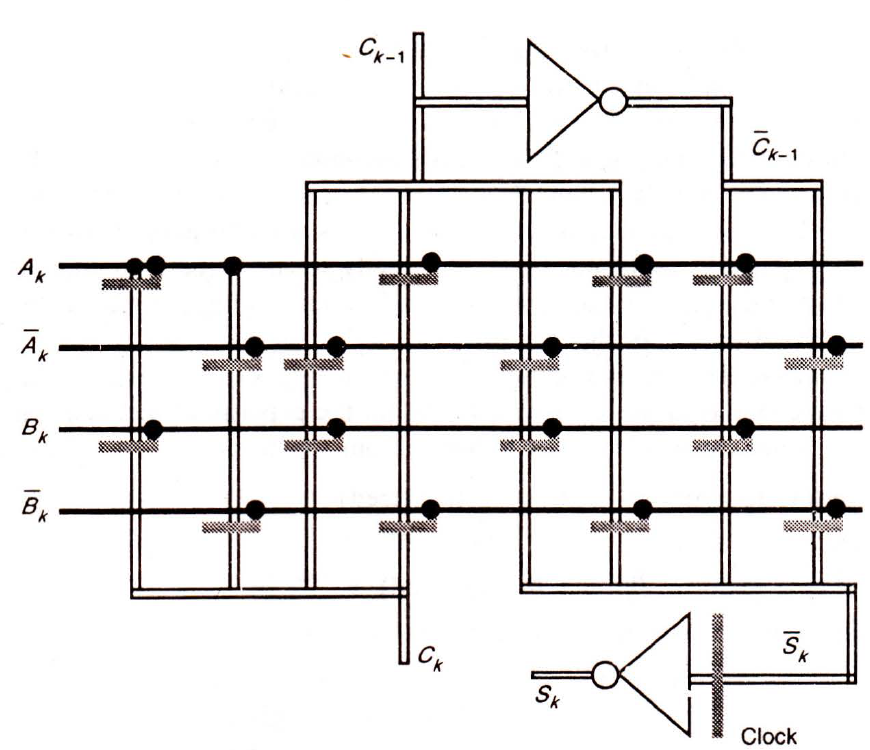
\includegraphics[width=0.89\linewidth]{Images/1}
		\caption{Multiplexer (n-switches)-based adder logic with stored and buffered sum output.}
		\label{fig:sk}
	\end{figure}
	The adder requirements can be stated as:
	
	\begin{enumerate}
		\item If $A_k = B_k$, then $S_k = C_{k-1}$,
		\item Else, $S_k = \overline{C}_{k-1}$.
	\end{enumerate}
	
	Similarly, for the carry $C_k$:
	
	\begin{enumerate}
		\item If $A_k = B_k$, then $C_k = A_k = B_k$,
		\item Else, $C_k = C_{k-1}$.
	\end{enumerate}
	
	Alternatively, the carry condition can be summarized as:
	
	\begin{enumerate}
		\item $C_k = 1$ when $A_k = B_k = 1$,
		\item $C_k = 0$ when $A_k = B_k = 0$.
	\end{enumerate}
	\newpage
	\section{Schematic Layout }
	
\begin{figure}[H]
	\centering
	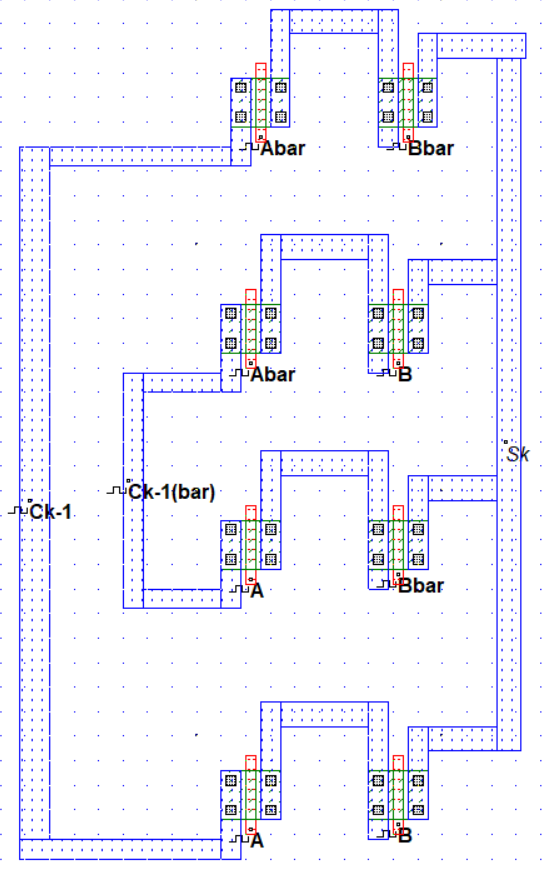
\includegraphics[width=0.89\linewidth]{Images/sk}
	\caption{Design of Sum (Sk) for ALU}
	\label{fig:sk}
\end{figure}
\begin{figure}[H]
	\centering
	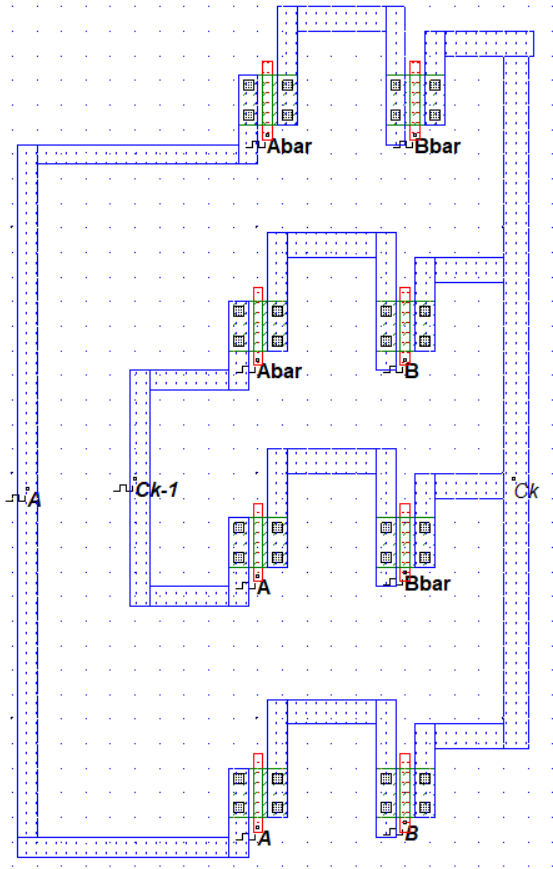
\includegraphics[width=0.89\linewidth]{Images/ck}
	\caption{Design of Carry (Ck) for ALU}
	\label{fig:sk}
\end{figure}

	\newpage
	\section{Specification}
		\begin{table}[H]
		\centering
		\caption{MOSFET Dimensions for nMOS and pMOS Transistors}
		\label{tab:MOSFET_dimensions}
		\begin{tabular}{|c|c|c|c|c|}
			\hline
			\textbf{MOS} & \textbf{\begin{tabular}[c]{@{}c@{}}Width\\ ($\mu m$)\end{tabular}} & \textbf{\begin{tabular}[c]{@{}c@{}}Length\\ ($\mu m$)\end{tabular}} & \textbf{\begin{tabular}[c]{@{}c@{}}Width\\ ($\lambda$)\end{tabular}} & \textbf{\begin{tabular}[c]{@{}c@{}}Length\\ ($\lambda$)\end{tabular}} \\ \hline
			nMOS & 0.600 & 0.120 & 10 & 2 \\ \hline
			pMOS & 0.600 & 0.120 & 10 & 2 \\ \hline
		\end{tabular}
		
	\end{table}
	\subsection{Specifications of ALU}
	\begin{table}[H]
		\centering
		\caption{Parameters of Input Clock Signals for A,B Ck-1 \& Ck-1bar}
		% Sub-table (a)
		\begin{subtable}[t]{0.48\textwidth} % Adjusted width for each sub-table
			\centering
			\begin{tabular}{|c|c|c|}
				\hline
				\textbf{Parameter}          & \textbf{Value} & \textbf{Unit} \\ \hline
				High Level $(V)$            & 5.00           & $V$           \\ \hline
				Low Level $(V)$             & 0.00           & $V$           \\ \hline
				Time Low $(tl)$             & 1          & $ns$          \\ \hline
				Rise Time $(tr)$            & 0.001          & $ns$          \\ \hline
				Time High $(th)$            & 1          & $ns$          \\ \hline
				Fall Time $(tf)$            & 0.001          & $ns$          \\ \hline
			\end{tabular}
			\caption{Input clock signal of A} % Sub-table (a) caption
		\end{subtable}
		\hfil
		% Sub-table (b)
		\begin{subtable}[t]{0.48\textwidth} % Adjusted width for each sub-table
			\centering
			\begin{tabular}{|c|c|c|}
				\hline
				\textbf{Parameter}          & \textbf{Value} & \textbf{Unit} \\ \hline
				High Level $(V)$            & 0.00           & $V$           \\ \hline
				Low Level $(V)$             & 5.00           & $V$           \\ \hline
				Time Low $(tl)$             & 1         & $ns$          \\ \hline
				Rise Time $(tr)$            & 0.001          & $ns$          \\ \hline
				Time High $(th)$            & 1          & $ns$          \\ \hline
				Fall Time $(tf)$            & 0.001          & $ns$          \\ \hline
			\end{tabular}
			\caption{Input clock signal of Abar} % Sub-table (b) caption
		\end{subtable}
		
		\begin{subtable}[t]{0.48\textwidth} % Adjusted width for each sub-table
			\centering
			\begin{tabular}{|c|c|c|}
				\hline
				\textbf{Parameter}          & \textbf{Value} & \textbf{Unit} \\ \hline
				High Level $(V)$            & 5.00           & $V$           \\ \hline
				Low Level $(V)$             & 0.00           & $V$           \\ \hline
				Time Low $(tl)$             & 2        & $ns$          \\ \hline
				Rise Time $(tr)$            & 0.001          & $ns$          \\ \hline
				Time High $(th)$            & 2          & $ns$          \\ \hline
				Fall Time $(tf)$            & 0.001          & $ns$          \\ \hline
			\end{tabular}
			
			\caption{Input clock signal of B} % Sub-table (a) caption
		\end{subtable}
		\hfil
		\begin{subtable}[t]{0.48\textwidth} % Adjusted width for each sub-table
			\centering
			\begin{tabular}{|c|c|c|}
				\hline
				\textbf{Parameter}          & \textbf{Value} & \textbf{Unit} \\ \hline
				High Level $(V)$            & 0.00           & $V$           \\ \hline
				Low Level $(V)$             & 5.00           & $V$           \\ \hline
				Time Low $(tl)$             & 2          & $ns$          \\ \hline
				Rise Time $(tr)$            & 0.001          & $ns$          \\ \hline
				Time High $(th)$            & 2         & $ns$          \\ \hline
				Fall Time $(tf)$            & 0.001          & $ns$          \\ \hline
			\end{tabular}
			
			\caption{Input clock signal of Bbar} % Sub-table (a) caption
		\end{subtable}
		
		
		\begin{subtable}[t]{0.48\textwidth} % Adjusted width for each sub-table
			\centering
			\begin{tabular}{|c|c|c|}
				\hline
				\textbf{Parameter}          & \textbf{Value} & \textbf{Unit} \\ \hline
				High Level $(V)$            & 5.00           & $V$           \\ \hline
				Low Level $(V)$             & 0.00           & $V$           \\ \hline
				Time Low $(tl)$             & 4        & $ns$          \\ \hline
				Rise Time $(tr)$            & 0.001          & $ns$          \\ \hline
				Time High $(th)$            & 4          & $ns$          \\ \hline
				Fall Time $(tf)$            & 0.001          & $ns$          \\ \hline
			\end{tabular}
			
			\caption{Input clock signal of Ck-1} % Sub-table (a) caption
		\end{subtable}
		\hfil
		\begin{subtable}[t]{0.48\textwidth} % Adjusted width for each sub-table
			\centering
			\begin{tabular}{|c|c|c|}
				\hline
				\textbf{Parameter}          & \textbf{Value} & \textbf{Unit} \\ \hline
				High Level $(V)$            & 0.00           & $V$           \\ \hline
				Low Level $(V)$             & 5.00           & $V$           \\ \hline
				Time Low $(tl)$             & 4          & $ns$          \\ \hline
				Rise Time $(tr)$            & 0.001          & $ns$          \\ \hline
				Time High $(th)$            & 4         & $ns$          \\ \hline
				Fall Time $(tf)$            & 0.001          & $ns$          \\ \hline
			\end{tabular}
			
			\caption{Input clock signal of Ck-1bar} % Sub-table (a) caption
		\end{subtable}
	\end{table}
	
	\begin{table}[H]
		\centering
		\caption{Parameters for Vdd+ and Vss- }
		\begin{tabular}{|c|c|c|}
			\hline
			\textbf{Parameter} & \textbf{Value} & \textbf{Unit} \\ \hline
			Vdd+               & 5.00           & $V $            \\ \hline
			Vss-               & 0.00           & $V$             \\ \hline
		\end{tabular}
		
	\end{table}
	\section{Output Waveshape }
\begin{figure}[H]
	\centering
	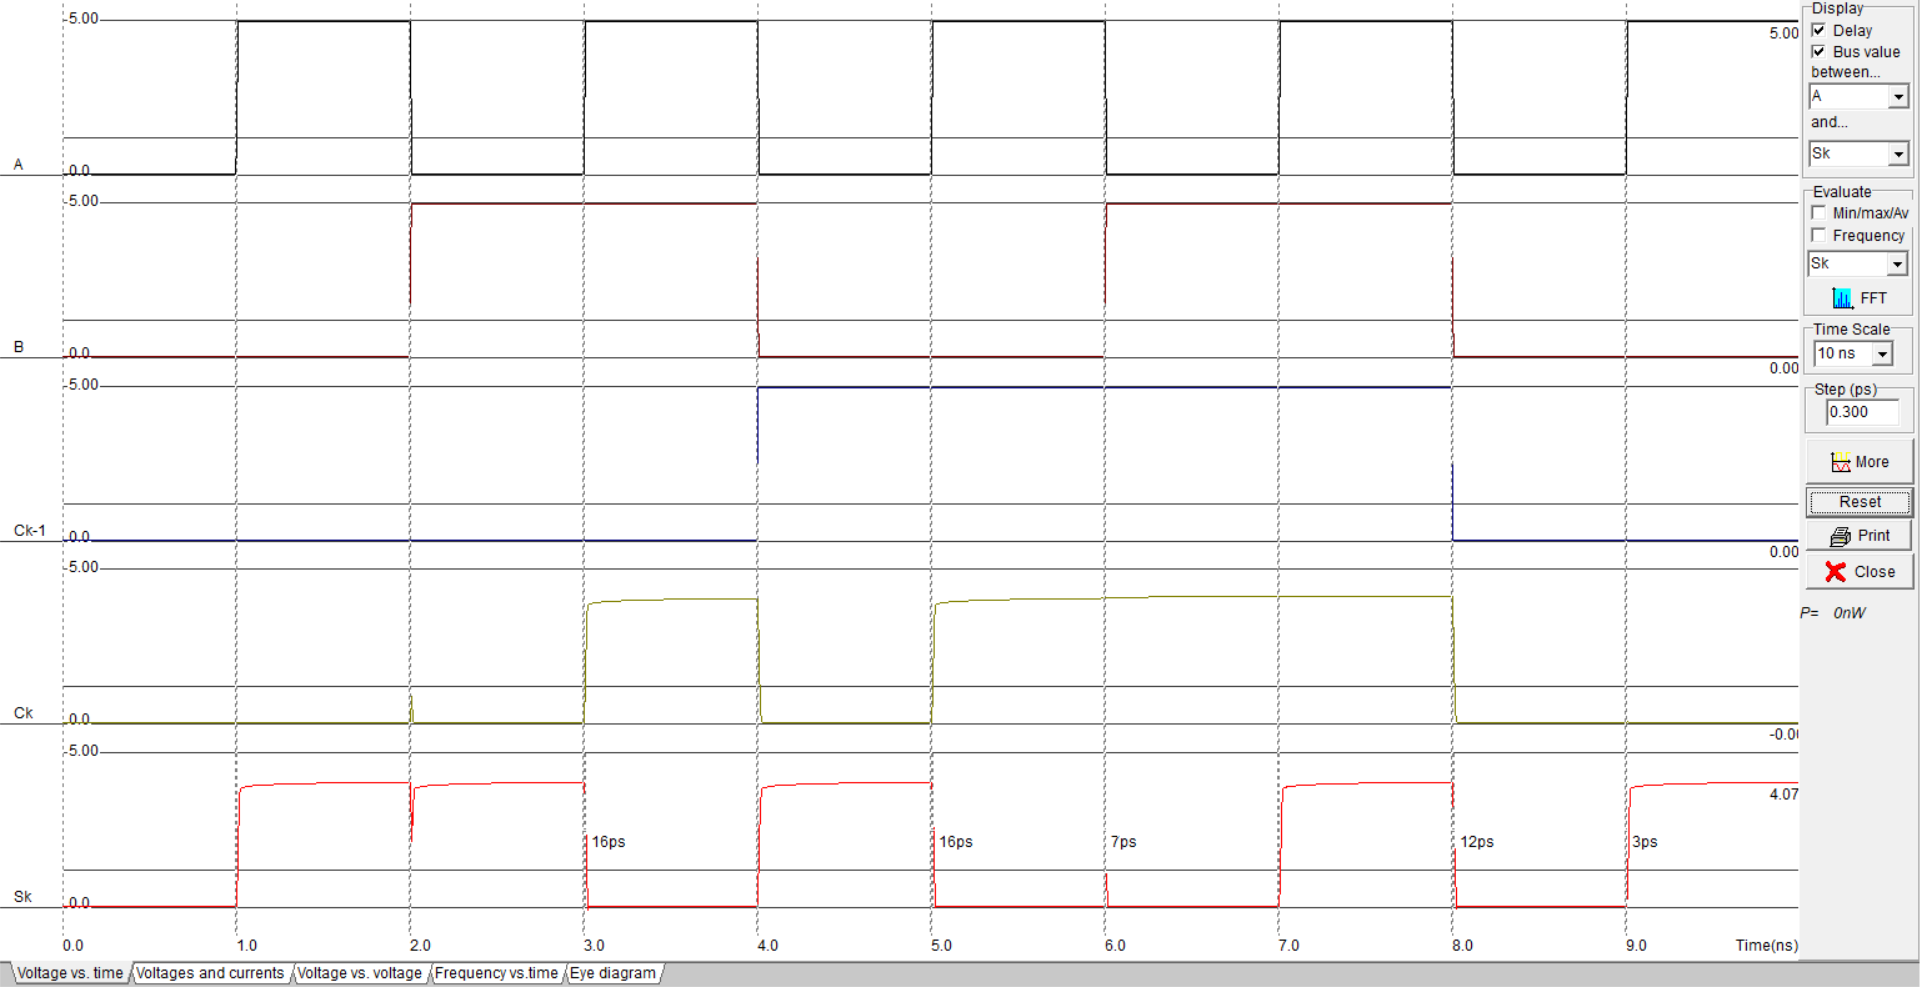
\includegraphics[width=1\linewidth, height=0.45\textheight]{Images/w}
	\caption{Output Waveshape of 4-Bit ALU}
	\label{fig:1}
\end{figure}
\section{Discussion}

In this experiment, the design and implementation of a 4-bit Arithmetic Logic Unit (ALU) were carried out using NMOS pass transistor logic. The operation of addition was successfully performed.
The ALU's functionality was derived based on standard logic equations for arithmetic operations. For addition, the sum ($S_k$) and carry ($C_k$) were calculated using truth tables and equations to ensure correctness for all possible input combinations. The sum ($S_k$) and carry ($C_k$) were implemented using nMOS transistors. Specifically, for the sum ($S_k$), the following logic was applied.If $A_k = B_k$, then $S_k = C_{k-1}$.
 Otherwise, $S_k = \overline{C}_{k-1}$.Similarly, the carry ($C_k$) was determined.If $A_k = B_k$, then $C_k = A_k = B_k$.
 Otherwise, $C_k = C_{k-1}$.\\
The behavior of the ALU was verified by testing various input conditions.The use of nMOS pass transistor logic resulted in a compact and efficient design. However, some fluctuations were noted during the implementation due to fast and sharp input transitions, which slightly affected the ALU's stability in certain cases.
Overall, the experiment demonstrated the feasibility of designing an ALU using nMOS pass transistor logic, providing insights into transistor-level implementation of arithmetic operations.

	
\end{document}